\documentclass[10pt,twocolumn]{article}
\usepackage[T1]{fontenc}
\usepackage[utf8]{inputenc}
\usepackage{microtype}
\usepackage[top=2.0cm,bottom=2.0cm,left=1.7cm,right=1.7cm,
            columnsep=0.65cm]{geometry}
\usepackage{mathpazo}
\usepackage{helvet}
\usepackage{courier}
\usepackage{parskip}
\setlength{\parskip}{4pt}
\usepackage[dvipsnames,table,xcdraw]{xcolor}
 
%% Colour palette
\definecolor{jpbiBlue}{RGB}{10,58,112}
\definecolor{jpbiMid}{RGB}{0,90,160}
\definecolor{jpbiLight}{RGB}{218,232,252}
\definecolor{jpbiAccent}{RGB}{0,140,186}
\definecolor{jpbiGreen}{RGB}{0,115,70}
\definecolor{jpbiRed}{RGB}{175,30,30}
\definecolor{jpbiOrange}{RGB}{210,105,30}
\definecolor{tableHead}{RGB}{10,58,112}
\definecolor{rowA}{RGB}{238,245,255}
\definecolor{rowB}{RGB}{255,255,255}
\definecolor{noteGray}{RGB}{245,247,250}
 
\usepackage{graphicx}
\usepackage{tikz}
\usetikzlibrary{arrows.meta,positioning,calc,shapes.geometric,
                backgrounds,shadows.blur,fit,decorations.pathreplacing}
\usepackage{pgfplots}
\pgfplotsset{compat=1.18}
\usepackage{booktabs,tabularx,multirow,makecell,array,longtable}
\renewcommand{\arraystretch}{1.28}
\usepackage{amsmath,amssymb,mathtools}
\usepackage[colorlinks=true,linkcolor=jpbiBlue,citecolor=jpbiMid,
            urlcolor=jpbiAccent,breaklinks=true]{hyperref}
\usepackage{float,placeins,stfloats}
\raggedbottom
 
%% Allow LaTeX to pack pages tightly with floats
\renewcommand{\topfraction}{0.95}
\renewcommand{\bottomfraction}{0.95}
\renewcommand{\textfraction}{0.05}
\renewcommand{\floatpagefraction}{0.80}
\renewcommand{\dbltopfraction}{0.95}
\renewcommand{\dblfloatpagefraction}{0.80}
\setcounter{topnumber}{4}
\setcounter{bottomnumber}{4}
\setcounter{totalnumber}{8}
\setcounter{dbltopnumber}{4}
\usepackage[font=small,labelfont=bf,labelsep=period,
            justification=justified,singlelinecheck=false]{caption}
\usepackage{enumitem}
\usepackage{fancyhdr,lastpage}
\usepackage{titlesec}
\usepackage{tcolorbox}
\tcbuselibrary{skins,breakable}
\usepackage{pifont}
\usepackage{xspace}
\usepackage{mdframed}
\usepackage{listings}
\usepackage{algorithm}
 
%% ── Headers / Footers ─────────────────────────────────────
\pagestyle{fancy}\fancyhf{}
\renewcommand{\headrulewidth}{0.4pt}
\renewcommand{\footrulewidth}{0.4pt}
\fancyhead[R]{\footnotesize\color{jpbiBlue}
  \textit{Front. Endocrinol. 2026}}
\fancyhead[L]{\footnotesize\color{jpbiBlue}
  \textit{ML Outcome Severity in Pediatric Endocrine Pharmacotherapy}}
\fancyfoot[R]{\footnotesize\color{gray}
  Page~\thepage~of~\pageref{LastPage}}
\fancyfoot[L]{\footnotesize\color{gray}
  \textit{Frontiers in Endocrinology | 2026 | Original Research Article}}
 
%% ── Section styles ────────────────────────────────────────
\titleformat{\section}
  {\large\bfseries\color{jpbiBlue}}{\thesection.}{0.5em}{}
  [\color{jpbiBlue}\rule{\linewidth}{0.8pt}\vspace{1pt}]
\titleformat{\subsection}
  {\normalsize\bfseries\color{jpbiMid}}{\thesubsection}{0.5em}{}
\titleformat{\subsubsection}
  {\small\bfseries\itshape\color{jpbiAccent}}
  {\thesubsubsection}{0.5em}{}
\titlespacing*{\section}{0pt}{10pt}{5pt}
\titlespacing*{\subsection}{0pt}{7pt}{3pt}
\titlespacing*{\subsubsection}{0pt}{5pt}{2pt}
 
%% ── Custom commands ───────────────────────────────────────
\newcommand{\FAERS}{\textsf{FAERS}\xspace}
\newcommand{\etal}{\textit{et al.}\xspace}
\newcommand{\cmark}{{\color{jpbiGreen}\ding{51}}}
\newcommand{\xmark}{{\color{jpbiRed}\ding{55}}}
 
%% ── tcolorbox styles ──────────────────────────────────────
\tcbset{
  absbox/.style={enhanced,breakable,
    colback=jpbiLight!55,colframe=jpbiBlue,
    boxrule=0.7pt,arc=3pt,
    left=6pt,right=6pt,top=2pt,bottom=2pt},
  cpybox/.style={enhanced,
    colback=jpbiBlue!5,colframe=jpbiBlue!60,
    boxrule=0.5pt,arc=2pt,
    left=5pt,right=5pt,top=4pt,bottom=4pt},
  findbox/.style={enhanced,breakable,
    colback=jpbiGreen!6,colframe=jpbiGreen!60,
    boxrule=0.5pt,arc=2pt,
    left=5pt,right=5pt,top=4pt,bottom=4pt,
    fonttitle=\small\bfseries\color{jpbiGreen}},
  sumtitle/.style={enhanced,
    colback=jpbiBlue!8,colframe=jpbiBlue,
    boxrule=0.7pt,arc=3pt,
    left=4pt,right=4pt,top=3pt,bottom=3pt}
}
 
%% ── Title block (journal format) ──────────────────────────
\makeatletter
\def\@maketitle{%
\newpage
\begin{center}
\leavevmode
{\color{jpbiBlue}\rule{\textwidth}{2pt}}\\[0.5pt]
{\Large\bfseries\color{jpbiBlue}
  FRONTIERS IN\\
  ENDOCRINOLOGY}\\[0pt]
{\small\itshape\color{jpbiMid}
  Manuscript submitted for peer review\enspace|\enspace
  2026\enspace|\enspace
  Preprint version --- not yet accepted}\\[0.5pt]
{\color{jpbiBlue}\rule{\textwidth}{0.5pt}}\\[0.5pt]
{\footnotesize\color{jpbiAccent}
  \MakeUppercase{Original Research Article}}\\[0.5pt]
{\color{jpbiBlue}\rule{\textwidth}{0.5pt}}\\[1pt]
%% ── Full Title ────────────────────────────────────────────
{\LARGE\bfseries\color{jpbiBlue}
  Machine Learning-Based Reported Outcome Severity Classification in\\
  Pediatric Growth and Endocrine Pharmacotherapy:\\
  A FAERS Cohort Study (2021--2025)}\\[2pt]
%% ── Authors with affiliations ─────────────────────────────
{\small
  \textbf{Atherv Telkar}$^{1,*}$\quad
  \textbf{Amey Telkar}$^{1,*}$\quad
  \textbf{Akshay Javalgikar}$^{2}$\quad
  \textbf{Nitin Madanwale}$^{2}$\quad
  \textbf{Darshan Ruikar}$^{1}$\quad
  \textbf{Preethi Baligar}$^{1}$}\\[2pt]
%% ── Affiliations ──────────────────────────────────────────
{\scriptsize
  $^{1}$School of Computing,\quad $^{2}$School of Pharmacy,\\
  MIT Vishwaprayag University, Solapur, Maharashtra, India\\[0pt]
  $^{*}$Equal primary authorship. These authors contributed
  equally as co-first authors.}\\[1pt]
{\scriptsize\itshape
  \textbf{Corresponding Authors:}\enspace
  Atherv Telkar
  (\href{mailto:athervtelkar08@gmail.com}
  {\texttt{athervtelkar08@gmail.com}});\quad
  Amey Telkar
  (\href{mailto:ameytelkar08@gmail.com}
  {\texttt{ameytelkar08@gmail.com}})}\\[2pt]
%% ── Front-matter statements ──────────────────────────────
{\scriptsize\color{black!80}
  \textbf{Funding:} None.\quad|\quad
  \textbf{Conflict of Interest:} None.\quad|\quad
  \textbf{Ethics:} Publicly available, de-identified FDA \FAERS data (45\,CFR\,\S\,46.104(d)(4)).\quad|\quad
  \textbf{Data Availability:} Publicly available at \href{https://fis.fda.gov/extensions/FPD-QDE-FAERS/FPD-QDE-FAERS.html}{fis.fda.gov/extensions/FPD-QDE-FAERS}.}\\[1pt]
{\color{jpbiBlue}\rule{\textwidth}{1.5pt}}
\end{center}}
\makeatother
 
%================================================================
\begin{document}
%================================================================
 
%% One-column title + abstract + key points all on page 1
\onecolumn
\enlargethispage{1.5cm}
\makeatletter\@maketitle\makeatother
 
\begin{tcolorbox}[absbox, title={Structured Abstract}, colbacktitle=jpbiBlue!8, coltitle=jpbiBlue, fonttitle=\small\bfseries\centering\MakeUppercase, toptitle=2pt, bottomtitle=2pt, top=1.5pt, bottom=1.5pt]
\footnotesize
\noindent\textbf{Background and Purpose:}
Post-marketing surveillance in pediatric endocrine pharmacotherapy remains almost entirely descriptive. No supervised machine-learning framework exists for multiclass outcome-severity classification in pediatric endocrine \FAERS reports. This study benchmarks tabular machine-learning classifiers for seven-class outcome-severity prediction in a large pediatric endocrine cohort.

\par\vspace{1.5pt}\noindent\textbf{Methods:}
\FAERS quarterly files (2021Q1--2025Q4, 20 quarters) were processed through a 13-step cleaning pipeline, deduplicated per FDA guidance, and restricted to ages 0--17 years (ICH E11(R1)). A unified cohort of $N = 44{,}431$ unique pediatric cases was constructed across five drug classes: Somatropin ($n = 31{,}948$), Levothyroxine ($n = 6{,}523$), Hydrocortisone ($n = 5{,}035$), Leuprolide ($n = 1{,}970$), and Methimazole ($n = 283$). The seven-class target (\texttt{outc\_cod}), missing in 73.56\% of records, was resolved via two-stage clinical imputation (AE-specific mode followed by clinical-indicator fallback). Random Forest and XGBoost were evaluated under stratified 80/20 leakage-aware holdout.

\par\vspace{1.5pt}\noindent\textbf{Results:}
XGBoost achieved 87.28\% accuracy (Macro-F1 0.4903) on the leakage-aware 14-column model, marginally outperforming Random Forest (86.99\%, Macro-F1 0.4889). The sanity-check 15-column model reached 97.47\% accuracy (Macro-F1 0.9704), confirming encoding integrity. Class distribution was highly imbalanced: OT 80.97\%, HO 13.18\%, DE 2.35\%, LT 2.46\%, CA 0.66\%, DS 0.35\%, RI 0.02\%. Device-related reports from injectable growth hormone delivery dominated the adverse-event landscape.

\par\vspace{1.5pt}\noindent\textbf{Conclusions:}
The 13-step preprocessing pipeline and two-stage imputation scheme generalise from adolescent metabolic pharmacotherapy to the full pediatric spectrum (0--17 years) with higher missingness (73.56\% vs 50.71\%). The framework represents a reproducible proof of concept for pharmacovigilance severity triage. External validation and prospective assessment are required before clinical deployment.

\par\vspace{1.5pt}\noindent\textbf{Keywords:}
Pharmacovigilance; FAERS; Pediatric Endocrinology; Growth Hormone; XGBoost; Outcome Severity Classification; Clinical Imputation.
\end{tcolorbox}
\twocolumn
 
%================================================================
\section{Introduction}
%================================================================
 
\subsection{Pediatric Endocrine Pharmacotherapy and Post-Marketing Surveillance}
 
Pediatric endocrine disorders --- including growth hormone deficiency (GHD), hypothyroidism, hyperthyroidism, central precocious puberty (CPP), and adrenal insufficiency --- collectively represent one of the most pharmacologically diverse therapeutic areas in pediatric medicine. Recombinant human growth hormone (rhGH) alone is approved for at least eight distinct pediatric indications, ranging from classical GHD and Turner syndrome to Prader--Willi syndrome and idiopathic short stature~\cite{grimberg2016}. The advent of long-acting growth hormone preparations (e.g.\ Ngenla, somapacitan) has further expanded the pediatric prescribing landscape~\cite{saenger2023}. Levothyroxine remains the standard of care for congenital and acquired hypothyroidism, with dosing adjustments required throughout childhood growth~\cite{biondi2019}. GnRH agonists such as leuprolide are the cornerstone treatment for CPP, with an expanding evidence base supporting their safety profile in younger populations~\cite{carel2009}. Hydrocortisone serves as the primary glucocorticoid replacement for congenital adrenal hyperplasia (CAH) and secondary adrenal insufficiency~\cite{bornstein2016}, while methimazole is the preferred anti-thyroid agent for pediatric Graves' disease~\cite{rivkees2014}.
 
Despite this pharmacological breadth, adverse drug reactions (ADRs) in pediatric endocrine pharmacotherapy remain under-characterised relative to metabolic pharmacotherapy (anti-obesity and anti-diabetic agents). Drug safety surveillance in pediatric populations requires particular caution because of age-dependent differences in pharmacokinetics, pharmacodynamics, and organ maturation, and because clinical trial populations rarely capture the full heterogeneity of real-world pediatric drug exposure~\cite{kearns2003}. This developmental sensitivity is especially relevant for endocrine agents: growth hormone therapy spans the entire pediatric age range from infancy through adolescence, with dose-response and safety profiles that differ substantially across ICH E11(R1) age bands~\cite{ich2017}.
 
The U.S. Food and Drug Administration's Adverse Event Reporting System (\FAERS) is the largest publicly available spontaneous-reporting pharmacovigilance database and has been widely used to characterize post-marketing adverse-event (AE) patterns in pediatric populations~\cite{misu2023, chen2022}. However, most \FAERS-based pediatric pharmacovigilance studies to date apply case/non-case disproportionality methods (reporting odds ratio, proportional reporting ratio, Bayesian Confidence Propagation Neural Network) that quantify statistical association between a drug and an AE term, rather than predicting the clinical severity of an individual reported outcome from the case-level feature profile. Systematic analyses of adverse event completeness in spontaneous reporting also highlight that outcome labels are frequently missing, creating a critical data quality challenge for any supervised learning approach~\cite{misu2023}.
 
In our prior work, we developed and validated a computational pharmacovigilance framework for multiclass outcome-severity classification specifically in the ICH E11(R1) adolescent age band (12--17 years) covering anti-obesity and anti-diabetic pharmacotherapy~\cite{telkar2026obesity}. That study benchmarked Random Forest, XGBoost, and a Heterogeneous Graph Attention Network (HANConv) across four nested cohorts ($N = 342$--$11{,}701$) and demonstrated that XGBoost achieved the strongest minority-class discrimination in larger cohorts (macro-F1 0.6250 on $N = 11{,}701$). The present study extends this framework to a distinct pharmacological domain --- growth and endocrine pharmacotherapy --- and to the full pediatric age spectrum (0--17 years), testing the generalisability of the 13-step preprocessing pipeline, two-stage clinical imputation, and tabular machine-learning approach.
 
No study, to our knowledge, has directly applied supervised machine-learning models for multiclass, case-level outcome-severity prediction within a cohort restricted to pediatric patients (0--17 years) receiving growth and endocrine pharmacotherapy. This represents both a methodological gap (whether the imputation and feature-engineering pipeline generalises to a pharmacologically distinct therapeutic class with markedly different adverse-event profiles) and a translational one (whether an interpretable severity-triage framework can be built for a pediatric endocrine drug-safety context where device-related adverse events dominate the reporting landscape).
 
This study contributes to computational pharmacovigilance by:
\begin{itemize}[leftmargin=*]
\item constructing a large pediatric \FAERS cohort (0--17 years) spanning 20 consecutive quarters (2021Q1--2025Q4) across five endocrine drug classes: Somatropin ($n = 31{,}948$), Levothyroxine ($n = 6{,}523$), Hydrocortisone ($n = 5{,}035$), Leuprolide ($n = 1{,}970$), and Methimazole ($n = 283$), yielding a total of $N = 44{,}431$ unique pediatric case reports;
\item demonstrating that the reproducible 13-step \FAERS preprocessing pipeline and two-stage clinical imputation scheme originally developed for adolescent metabolic pharmacotherapy~\cite{telkar2026obesity} generalises to a pharmacologically distinct therapeutic domain with substantially higher outcome-label missingness (73.56\% vs 50.71\%);
\item benchmarking Random Forest and XGBoost for seven-class reported outcome-severity classification (including Congenital Anomaly, which was absent from the adolescent metabolic cohorts); and
\item characterising the markedly different adverse-event landscape of pediatric endocrine pharmacotherapy, where device-related reports associated with injectable growth hormone delivery systems dominate the reporting profile.
\end{itemize}
 
The remainder of this article is organized as follows: Section~2 synthesizes related work and states the research gap; Section~3 details the data source, cohort construction, feature engineering, imputation, and model architectures; Section~4 reports cohort characteristics and predictive performance; Section~5 discusses interpretation, comparison with the broader literature, and study limitations; Section~6 concludes.
 
%================================================================
\section{Related Work}
%================================================================
 
\subsection{Prior Methodologies}
Surveillance and prediction methodologies in pediatric endocrine pharmacovigilance can be broadly categorized into three families: statistical disproportionality, tabular supervised machine learning, and graph-based approaches. Table~\ref{tab:related_work} synthesizes these approaches and highlights their limitations for cohort-specific outcome prediction in the endocrine domain.
 
\subsubsection{Disproportionality and Case/Non-Case Methods}
The dominant paradigm in pediatric pharmacovigilance remains statistical disproportionality analysis applied to case/non-case $2\times2$ contingency tables~\cite{vanpuijenbroek2002, rothman2004}. In the endocrine domain, these methods have been used to characterize safety signals for growth hormone therapy~\cite{bell2010}, GnRH agonists among different pediatric and adult age groups~\cite{stochholm2020}, and pediatric adverse drug events more broadly~\cite{chen2020thyroid}. While these methods are interpretable and well-established, they estimate drug-level AE association strength rather than predicting individual-report outcome severity.
 
\subsubsection{Tabular Supervised Machine Learning}
Ensemble tree methods --- Random Forest and gradient-boosted trees (XGBoost) --- have been widely adopted for structured pharmacovigilance signal detection and clinical outcome-prediction tasks~\cite{tian2025, farnoush2024}. Our prior work applied these methods specifically to adolescent metabolic pharmacotherapy on \FAERS~\cite{telkar2026obesity}. Their principal limitation for pharmacovigilance is that each case is treated as an independent feature vector, discarding the relational structure linking a given case to other cases through shared drug exposures and adverse-event terms.
 
\subsubsection{Graph-Based Methods}
Heterogeneous graph neural networks have been proposed for large-scale pharmacovigilance~\cite{gao2025, shi2026}, but have not been evaluated on endocrine-specific pediatric sub-cohorts. In our prior work, we found that HANConv GNN's accuracy advantage over tabular models was largely driven by majority-class prediction bias (macro-F1 $\le$ 0.3733 in cohorts $N \ge 5{,}000$)~\cite{telkar2026obesity}. Therefore, the present study focuses exclusively on tabular learners.
 
%% TABLE — Related Work Comparison
\begin{table*}[t]
\caption{Comparative positioning of prior pharmacovigilance methodologies against the proposed pediatric endocrine outcome prediction framework.}
\label{tab:related_work}
\centering\small\setlength{\tabcolsep}{5pt}
\begin{tabularx}{\textwidth}{|>{\raggedright\arraybackslash\hsize=0.7\hsize}X|>{\raggedright\arraybackslash\hsize=0.8\hsize}X|>{\raggedright\arraybackslash\hsize=1.0\hsize}X|>{\raggedright\arraybackslash\hsize=1.3\hsize}X|>{\raggedright\arraybackslash\hsize=1.3\hsize}X|>{\centering\arraybackslash\hsize=0.9\hsize}X|}
\hline
\rowcolor{tableHead}
\color{white}\textbf{Approach Type} & \color{white}\textbf{Representative Work} & \color{white}\textbf{Features/Data} & \color{white}\textbf{Strengths} & \color{white}\textbf{Limitations} & \color{white}\textbf{Resolves missing \texttt{outc\_cod}?}\\
\hline
\rowcolor{rowA} Disproportionality & Evans \etal~\cite{evans2001}, Bate \etal~\cite{bate1998} & Bipartite drug-ADR counts & Robust for global signal detection; low compute cost & Limited to pairwise associations; cannot handle multi-variable outcomes & \xmark\ (Requires complete labels) \\
\hline
\rowcolor{rowB} Tabular ML & Tian \etal~\cite{tian2025}, Farnoush \etal~\cite{farnoush2024} & Demographic + clinical features & Strong classification performance on dense tabular datasets & Discards incomplete reports; introduces selection bias & \xmark\ (Discards or uses \texttt{NS}) \\
\hline
\rowcolor{rowA} GH Safety Studies & Bell \etal~\cite{bell2010}, Stochholm \etal~\cite{stochholm2020} & Registry/FAERS descriptive & Disease-specific safety characterisation & No severity prediction; descriptive only & \xmark\ (Descriptive) \\
\hline
\rowcolor{rowB} Graph-Based Pharmacovigilance & Gao \etal~\cite{gao2025}, Shi \etal~\cite{shi2026} & Heterogeneous drug-patient-AE graphs & Captures relational structure between drugs, patients, and adverse events; global link prediction & Evaluated on adult populations only; not tested on pediatric endocrine sub-cohorts; high compute cost & \xmark\ (Requires complete labels) \\
\hline
\rowcolor{rowA} Pediatric ADE Surveillance & Misu \etal~\cite{misu2023}, Chen \etal~\cite{chen2020thyroid} & AE completeness review; pediatric ADE frequency & Highlights reporting gaps; age-stratified ADE characterisation & No ML classification; descriptive only; no outcome imputation & \xmark\ (Descriptive) \\
\hline
\rowcolor{jpbiLight}
\textbf{Proposed Framework} & \textbf{This Study} & \textbf{14 core clinical columns}* & \textbf{Full pediatric (0--17y); endocrine-specific; 87.28\% accuracy; clinical imputation resolving 73.56\% missingness} & \textbf{Cohort-specific tabular modeling; 7-class including CA} & \cmark\ (\textbf{2-Stage Imputation}) \\
\hline
\end{tabularx}
 
\smallskip
\noindent\footnotesize\textit{*Note: The 14 core clinical columns include 1 target variable; the primary leakage-aware predictive models utilize 13 clinical features. The 15-column set additionally includes \texttt{severity\_score} for ablation.}
\end{table*}
 
\subsection{Research Gap}
Despite these developments, no existing study has (i)~applied supervised tabular machine learning for multiclass outcome-severity classification to a \FAERS cohort restricted to the full pediatric age band (0--17 years) receiving growth and endocrine pharmacotherapy, (ii)~demonstrated the generalisability of a two-stage clinical imputation pipeline originally developed for adolescent metabolic pharmacotherapy to a pharmacologically distinct therapeutic domain with substantially higher outcome-label missingness, or (iii)~characterised how the dominant role of device-related adverse events in injectable endocrine pharmacotherapy (particularly rhGH) affects the outcome distribution and classification landscape relative to metabolic drug cohorts. This study directly addresses these gaps.
 
%================================================================
\section{Dataset and Study Population}
%================================================================
 
\subsection{Data Source and Deduplication Practice}
\FAERS is the FDA's primary database for post-marketing drug safety surveillance~\cite{fda2026}. It collects voluntary and mandatory spontaneous ADR reports from healthcare professionals, consumers, manufacturers, and distributors. For this study, quarterly data extract files spanning 20 consecutive quarters (Q1 2021 through Q4 2025) were obtained.
 
Each quarterly release of the raw database consists of seven dollar-sign-delimited ASCII text files, each capturing a distinct dimension of the adverse event report:
\begin{itemize}[leftmargin=*]
\item \textbf{DEMO (Demographic):} Patient demographics (age, gender, weight), report source characteristics, country of origin, and reporting dates. Selected features include \texttt{age\_years}, \texttt{sex}, \texttt{weight\_kg}, \texttt{occp\_cod}, \texttt{reporter\_country}, and \texttt{occr\_country}.
\item \textbf{DRUG (Drug Exposure):} Details on all medications reported for the event, including brand/generic names, suspect roles (\texttt{role\_cod}), routes of administration, dose amounts, units, dosage forms, and therapy sequence numbers (\texttt{drug\_seq}).
\item \textbf{REAC (Reactions):} Adverse events experienced by the patient, coded to MedDRA Preferred Terms (\texttt{pt\_term})~\cite{meddra2023}.
\item \textbf{OUTC (Outcomes):} Patient outcomes, categorized as death (\texttt{DE}), life-threatening (\texttt{LT}), hospitalization (\texttt{HO}), disability (\texttt{DS}), congenital anomaly (\texttt{CA}), required intervention (\texttt{RI}), or other serious (\texttt{OT}).
\item \textbf{THER (Therapy Dates):} Dates of drug therapy start and end.
\item \textbf{INDI (Indications):} Medical indications (\texttt{indi\_pt}) for which the drug was prescribed.
\item \textbf{RPSR (Report Source):} Administrative metadata on the reporting entity.
\end{itemize}
 
\textbf{Case Versioning and Deduplication:} For cases with multiple report versions sharing a common case identifier, the report with the most recent FDA receipt date was retained, with ties broken by the highest primary report identifier (\texttt{primaryid})~\cite{fda2026}. This deduplication convention is consistent with our prior methodology~\cite{telkar2026obesity} and follows the best-practice principles discussed in recent adverse event reporting quality reviews~\cite{misu2023}.
 
\textbf{Raw Counts and Column Attrition:} Across the 20 quarters, the raw \FAERS database contains approximately 8.75 million report submissions across all age groups. For the pediatric cohort (0--17 years) prescribed any of the target endocrine drugs, a total of 44{,}431 unique case reports remained after deduplication. Across the seven raw files, there are 62 columns. At Step~1, 18 columns are dropped because they are either highly sparse (${\geq}$75\% null) or redundant for outcome severity prediction. The remaining 44 columns, combined with join keys and derived features, constitute the analytical dataset.
 
%% TABLE — Raw vs Cleaned Column Counts
\begin{table}[htbp]
\caption{Raw vs.\ Cleaned Column Counts per \FAERS File.}
\label{tab:colcounts}
\centering\footnotesize\setlength{\tabcolsep}{4pt}
\begin{tabular}{|l|r|r|r|}
\hline
\rowcolor{tableHead}
\color{white}\textbf{File}&
\color{white}\textbf{Raw Cols.}&
\color{white}\textbf{Dropped}&
\color{white}\textbf{Kept}\\
\hline
\rowcolor{rowA}DEMO&22&9&13\\
\hline
\rowcolor{rowB}DRUG&19&8&11\\
\hline
\rowcolor{rowA}REAC&4&1&3\\
\hline
\rowcolor{rowB}OUTC&3&0&3\\
\hline
\rowcolor{rowA}THER&7&0&7\\
\hline
\rowcolor{rowB}INDI&4&0&4\\
\hline
\rowcolor{rowA}RPSR&3&0&3\\
\hline
\rowcolor{jpbiLight}
\textbf{TOTAL}&\textbf{62}&\textbf{18}&\textbf{44}\\
\hline
\end{tabular}
\end{table}
 
\subsection{Study Population and Cohort Definitions}
The study population was restricted to the full pediatric age band, defined as 0 to 17 completed years, encompassing all four ICH E11(R1) sub-bands~\cite{ich2017}: Neonate ($<\!28$d), Infant ($<\!2$y), Child (2--11y), and Adolescent (12--17y). A unified endocrine cohort was constructed from a pre-specified drug panel covering five growth and endocrine pharmacotherapy classes:
 
\begin{itemize}[leftmargin=*]
\item \textbf{Somatropin (7 brand/generic variants, $n = 31{,}948$ unique pediatric cases):} Genotropin, Omnitrope, Norditropin, Saizen, Nutropin AQ, Ngenla, and generic somatropin. This class represents recombinant human growth hormone (rhGH) prescribed for GHD, Turner syndrome, Prader--Willi syndrome, idiopathic short stature, and other approved indications.
\item \textbf{Levothyroxine (3 variants, $n = 6{,}523$ cases):} Levothyroxine, Levothyroxine sodium, and Synthroid. Standard thyroid hormone replacement for congenital and acquired hypothyroidism.
\item \textbf{Hydrocortisone (2 variants, $n = 5{,}035$ cases):} Hydrocortisone and Hydrocortisone/Lactate. Primary glucocorticoid replacement for congenital adrenal hyperplasia and secondary adrenal insufficiency.
\item \textbf{Leuprolide (5 variants, $n = 1{,}970$ cases):} Eligard, Leuprolide acetate, Fensolvi, Supprelin LA, and Triptodur. GnRH agonists used for central precocious puberty.
\item \textbf{Methimazole (1 variant, $n = 283$ cases):} Methimazole. Anti-thyroid agent for pediatric Graves' disease.
\end{itemize}
 
\textbf{Note on Patient Overlap:} The sum of individual drug-class counts ($31{,}948 + 6{,}523 + 5{,}035 + 1{,}970 + 283 = 45{,}759$) exceeds the total unique patient count of 44{,}431 because 1{,}328 patients (2.99\%) received medications from more than one endocrine drug class concurrently (e.g.\ a patient receiving both somatropin and levothyroxine for hypopituitarism). The total cohort count represents the set union of all five drug classes.
 
\textbf{Pediatric Representation and Denominator Context:} Across the 20-quarter study period, 606{,}302 total pediatric (0--17y) case reports of any indication were logged in \FAERS, of which 13{,}038 (2.15\%) carried an explicit endocrine-related indication code. The much larger panel count of 44{,}431 reflects that most qualifying exposures were captured by drug name irrespective of the coded indication.
 
\textbf{ICH E11(R1) Age Band Distribution:} The cohort spans all four pediatric sub-bands: Adolescent (12--17y, $n = 22{,}984$, 51.73\%), Child (2--11y, $n = 19{,}196$, 43.20\%), Infant ($<$2y, $n = 1{,}277$, 2.87\%), and Neonate ($<$28d, $n = 974$, 2.19\%). The adolescent and child bands together account for 94.93\% of the cohort, reflecting the age distribution of most endocrine pharmacotherapy indications.
 
\subsection{Patient Outcomes Distribution}
 
In addition to demographic and reaction data, \FAERS captures the clinical outcomes (OUTC) associated with each adverse event report. Figure~\ref{fig:outcomes} illustrates the distribution of reported outcome codes across the endocrine cohort.
 
\begin{figure}[htbp]
\hspace{0pt}
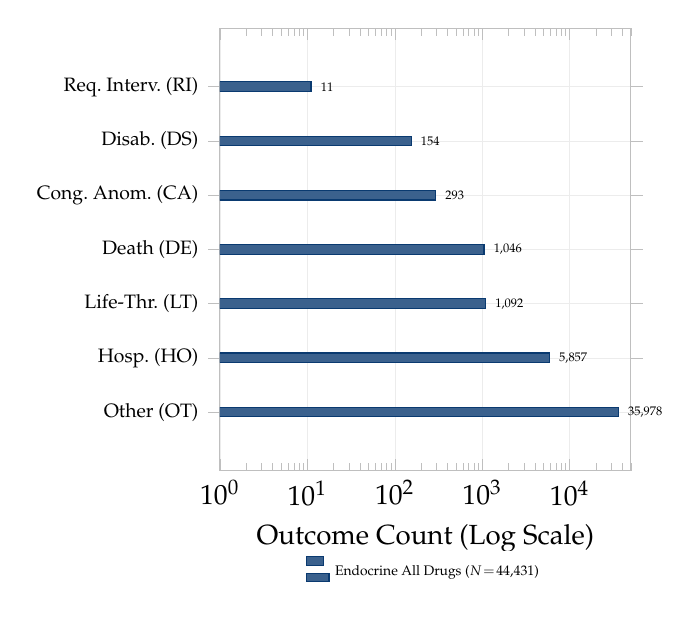
\begin{tikzpicture}
\begin{axis} [
  xbar,
  width=6.8cm, height=7.2cm,
  bar width=3.5pt,
  enlarge y limits=0.18,
  xmin=1, xmax=50000,
  xmode=log,
  xlabel={Outcome Count (Log Scale)},
  symbolic y coords={OT,HO,LT,DE,CA,DS,RI},
  ytick={OT,HO,LT,DE,CA,DS,RI},
  yticklabels={Other (OT), Hosp.\ (HO), Life-Thr.\ (LT), Death (DE), Cong.\ Anom.\ (CA), Disab.\ (DS), Req.\ Interv.\ (RI)},
  yticklabel style={font=\scriptsize, align=right},
  grid=major,
  grid style={line width=0.2pt,draw=gray!15},
  axis line style={color=gray!50},
  tick style={color=gray!50},
  legend style={at={(0.5,-0.18)}, anchor=north, legend columns=1, font=\tiny, draw=none},
]
%% Endocrine All Drugs (post-imputation)
\addplot[fill=jpbiBlue!80, draw=jpbiBlue,
  nodes near coords, point meta=explicit symbolic,
  every node near coord/.append style={font=\fontsize{4.5}{6}\selectfont, color=black, anchor=west}]
  coordinates {
  (35978,OT) [35,978]
  (5857,HO) [5,857]
  (1092,LT) [1,092]
  (1046,DE) [1,046]
  (293,CA) [293]
  (154,DS) [154]
  (11,RI) [11]
};
\addlegendentry{Endocrine All Drugs ($N\!=\!44{,}431$)}
\end{axis}
\end{tikzpicture}
\caption{Distribution of clinical outcomes in the pediatric endocrine cohort (post-imputation). Codes reflect the most severe outcome per report. A log scale accommodates the wide frequency range. Note the presence of Congenital Anomaly (CA, $n = 293$), which was absent from the adolescent metabolic cohorts in our prior work.}
\label{fig:outcomes}
\end{figure}
 
The majority of reports fall into the broad ``Other'' (OT) category (35{,}978, 80.97\%), reflecting the high proportion of device-related and non-serious adverse events in the growth hormone sub-panel. Hospitalisation (HO, $n = 5{,}857$, 13.18\%) is the second most common outcome. The presence of Congenital Anomaly (CA, $n = 293$, 0.66\%) distinguishes this cohort from the adolescent metabolic cohorts, where CA was entirely absent; this is clinically expected given the younger age distribution and the inclusion of neonates and infants. Required Intervention (RI, $n = 11$, 0.02\%) remains the rarest category.
 
%% TABLE — Quarter-Wise Counts
\begin{table*}[!t]
\caption{Quarter-wise FAERS reporting volume for the pediatric cohort (0--17 years) from 2021 to 2025 across the five endocrine drug classes. Individual drug-class columns may sum to more than the ``Endocrine All'' column due to patient overlap across drug classes.}
\label{tab:cohort_counts}
\centering\small\setlength{\tabcolsep}{4pt}
\begin{tabular}{|l|c|c|c|c|c|c|c|}
\hline
\rowcolor{tableHead}
\color{white}\textbf{Quarter} &
\color{white}\textbf{Pediatric} &
\color{white}\textbf{Endocrine} &
\color{white}\textbf{Endocrine} &
\color{white}\textbf{Somatropin} &
\color{white}\textbf{Levothyroxine} &
\color{white}\textbf{Hydrocortisone} &
\color{white}\textbf{Leuprolide}\\
\rowcolor{tableHead}
\color{white}\textbf{} &
\color{white}\textbf{Reports} &
\color{white}\textbf{Indication} &
\color{white}\textbf{All Drugs} &
\color{white}\textbf{Only} &
\color{white}\textbf{Only} &
\color{white}\textbf{Only} &
\color{white}\textbf{Only}\\
\hline
\rowcolor{rowA} 2021 Q1 & 28,359 & 291 & 855 & 400 & 204 & 231 & 43\\
\hline
\rowcolor{rowB} 2021 Q2 & 29,401 & 305 & 882 & 385 & 256 & 224 & 38\\
\hline
\rowcolor{rowA} 2021 Q3 & 25,312 & 367 & 1,180 & 572 & 236 & 262 & 147\\
\hline
\rowcolor{rowB} 2021 Q4 & 26,855 & 532 & 1,807 & 1,327 & 276 & 208 & 59\\
\hline
\rowcolor{rowA} 2022 Q1 & 27,683 & 543 & 1,959 & 1,405 & 331 & 226 & 35\\
\hline
\rowcolor{rowB} 2022 Q2 & 25,896 & 499 & 1,811 & 1,197 & 264 & 314 & 65\\
\hline
\rowcolor{rowA} 2022 Q3 & 27,166 & 434 & 1,637 & 968 & 326 & 291 & 91\\
\hline
\rowcolor{rowB} 2022 Q4 & 29,025 & 586 & 1,854 & 1,219 & 392 & 248 & 49\\
\hline
\rowcolor{rowA} 2023 Q1 & 29,901 & 568 & 1,818 & 1,136 & 405 & 231 & 85\\
\hline
\rowcolor{rowB} 2023 Q2 & 28,603 & 581 & 2,096 & 1,516 & 335 & 216 & 73\\
\hline
\rowcolor{rowA} 2023 Q3 & 28,690 & 641 & 2,257 & 1,563 & 365 & 249 & 133\\
\hline
\rowcolor{rowB} 2023 Q4 & 27,752 & 754 & 2,682 & 2,097 & 350 & 208 & 90\\
\hline
\rowcolor{rowA} 2024 Q1 & 29,564 & 897 & 3,297 & 2,782 & 306 & 223 & 85\\
\hline
\rowcolor{rowB} 2024 Q2 & 27,944 & 813 & 2,303 & 1,669 & 302 & 250 & 160\\
\hline
\rowcolor{rowA} 2024 Q3 & 31,009 & 714 & 2,010 & 1,322 & 298 & 254 & 179\\
\hline
\rowcolor{rowB} 2024 Q4 & 35,155 & 1,031 & 3,469 & 2,807 & 345 & 268 & 121\\
\hline
\rowcolor{rowA} 2025 Q1 & 33,387 & 1,103 & 3,530 & 2,746 & 322 & 287 & 256\\
\hline
\rowcolor{rowB} 2025 Q2 & 34,595 & 913 & 2,995 & 2,323 & 346 & 270 & 126\\
\hline
\rowcolor{rowA} 2025 Q3 & 40,612 & 764 & 3,086 & 2,294 & 433 & 323 & 72\\
\hline
\rowcolor{rowB} 2025 Q4 & 39,393 & 702 & 2,903 & 2,220 & 431 & 252 & 63\\
\hline
\rowcolor{jpbiLight}
\textbf{TOTAL} & \textbf{606,302} & \textbf{13,038} & \textbf{44,431} & \textbf{31,948} & \textbf{6,523} & \textbf{5,035} & \textbf{1,970}\\
\hline
\end{tabular}
 
\smallskip
\noindent\footnotesize\textit{Note: Methimazole Only ($n = 283$ total) is omitted from this table due to space constraints but is included in all analytical models. See Table~\ref{tab:baseline} for the complete demographic profile.}
\end{table*}
 
%% TABLE — Baseline Demographics
\begin{table*}[!t]
\caption{Baseline demographic and clinical characteristics of the pediatric endocrine cohort. All values computed from the imputed 14-column dataset ($N = 44{,}431$).}
\label{tab:baseline}
\centering\small\setlength{\tabcolsep}{5pt}
\begin{tabular}{|l|c|}
\hline
\rowcolor{tableHead}
\color{white}\textbf{Characteristic} &
\color{white}\textbf{Endocrine All Drugs}\\
\rowcolor{tableHead}
\color{white} &
\color{white}\textbf{(n=44,431)}\\
\hline
\rowcolor{rowA} Age, years, mean $\pm$ SD & $10.54 \pm 4.23$\\
\hline
\rowcolor{rowB} Age range & 0.0--17.0\\
\hline
\rowcolor{rowA} Age band: Adolescent (12--17y) & 22,984 (51.73\%)\\
\hline
\rowcolor{rowB} Age band: Child (2--11y) & 19,196 (43.20\%)\\
\hline
\rowcolor{rowA} Age band: Infant ($<$2y) & 1,277 (2.87\%)\\
\hline
\rowcolor{rowB} Age band: Neonate ($<$28d) & 974 (2.19\%)\\
\hline
\rowcolor{rowA} Sex, Male & 24,717 (55.63\%)\\
\hline
\rowcolor{rowB} Sex, Female & 18,491 (41.62\%)\\
\hline
\rowcolor{rowA} Sex, missing & 1,223 (2.75\%)\\
\hline
\rowcolor{rowB} Drug role, primary suspect (PS) & 34,337 (77.28\%)\\
\hline
\rowcolor{rowA} Drug role, secondary suspect (SS) & 12,954 (29.16\%)\\
\hline
\rowcolor{rowB} Drug role, concomitant (C) & 8,864 (19.95\%)\\
\hline
\rowcolor{rowA} Drug role, interacting (I) & 52 (0.12\%)\\
\hline
\rowcolor{rowB} Fatal outcome (DE) & 1,046 (2.35\%)\\
\hline
\rowcolor{rowA} Serious outcome (HO+LT+DE+DS) & 8,149 (18.34\%)\\
\hline
\rowcolor{rowB} Weight (\texttt{weight\_kg}) missing & 73.62\%\\
\hline
\rowcolor{rowA} Indication (\texttt{indi\_pt}) missing & 49.16\%\\
\hline
\rowcolor{rowB} Top indication: Growth hormone deficiency & 6,601 (14.86\%)\\
\hline
\rowcolor{rowA} Top indication: Short stature & 2,998 (6.75\%)\\
\hline
\rowcolor{rowB} Top indication: Hypopituitarism & 1,847 (4.16\%)\\
\hline
\rowcolor{rowA} Primary route: Subcutaneous & 11,524 (25.94\%)\\
\hline
\end{tabular}
\end{table*}
 
%================================================================
\section{Methodology}
%================================================================
 
\subsection{Problem Formulation}
Let $D$ represent a dataset of adverse event reports. Each report $r_i \in D$ is characterized by a feature vector $\mathbf{x}_i \in \mathbb{R}^d$ comprising $d=13$ clinical and demographic features, and a target outcome label $y_i \in Y$, where $Y = \{\texttt{CA}, \texttt{DE}, \texttt{DS}, \texttt{HO}, \texttt{LT}, \texttt{OT}, \texttt{RI}\}$ represents the set of seven serious clinical outcomes. The goal is to learn a mapping function $f: \mathbf{x}_i \to y_i$ that maximizes multiclass classification accuracy and Macro-F1 under leakage-aware evaluation. Unlike our prior metabolic pharmacotherapy study, which involved six outcome classes (CA was absent), the endocrine cohort includes Congenital Anomaly (CA, $n = 293$) due to the inclusion of neonates and infants.
 
\subsection{Data Cleaning and Preprocessing Pipeline (13 Steps)}
\label{sec:pipeline}
 
The cohort is extracted from raw quarterly FDA \FAERS files through the same validated 13-step cleaning pipeline originally developed and described in our prior work~\cite{telkar2026obesity}, illustrated in Figure~\ref{fig:framework_overview}. The pipeline is deterministic and auditable, with the \textbf{Approve/Reject gate at Step~13} ensuring that nothing enters the analysis database until a human reviewer reads through the generated Preview Report and clicks Approve.
 
\begin{figure*}[htbp]
\centering
\resizebox{\textwidth}{!}{%
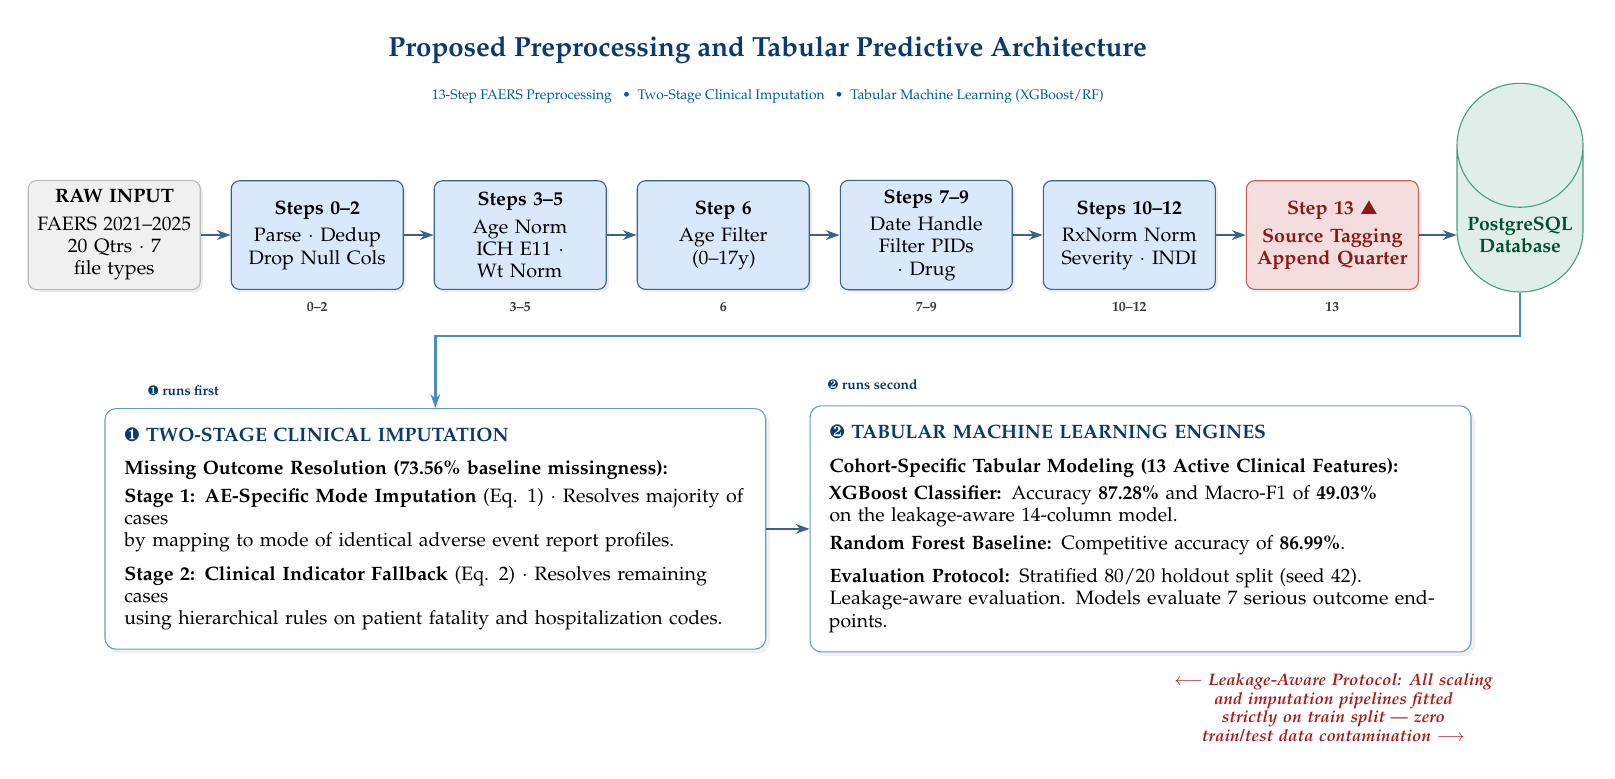
\begin{tikzpicture}[
  font=\scriptsize,
  pipebox/.style={rectangle,rounded corners=3pt,
    draw=jpbiBlue!80,fill=jpbiLight,
    minimum width=2.05cm,minimum height=1.38cm,
    align=center,text width=1.95cm,
    drop shadow={shadow xshift=1pt,shadow yshift=-1pt,
    opacity=0.15}},
  rawbox/.style={pipebox,fill=gray!12,draw=gray!55},
  gatebox/.style={pipebox,fill=jpbiRed!15,draw=jpbiRed!70,
    font=\scriptsize\bfseries,text=jpbiRed!80!black},
  dbbox/.style={cylinder,shape border rotate=90,
    draw=jpbiGreen!70,fill=jpbiGreen!12,
    minimum width=1.6cm,minimum height=1.15cm,
    align=center,
    font=\scriptsize\bfseries\color{jpbiGreen!70!black}},
  engine/.style={rectangle,rounded corners=4pt,
    draw=jpbiMid!60,fill=white,inner sep=7pt,align=left,
    drop shadow={shadow xshift=1.5pt,shadow yshift=-1.5pt,
    opacity=0.12}},
  arr/.style={-{Stealth[length=5pt,width=3.5pt]},
    line width=0.9pt,color=jpbiBlue!80},
  darr/.style={-{Stealth[length=5pt,width=3.5pt]},
    line width=0.9pt,color=jpbiMid!70},
]
\node[font=\normalsize\bfseries\color{jpbiBlue},align=center]
  (TIT) at (0,0)
  {Proposed Preprocessing and Tabular Predictive Architecture};
\node[font=\tiny\color{jpbiMid},align=center,
  below=2pt of TIT] (SUB)
  {13-Step FAERS Preprocessing \enspace\textbullet\enspace Two-Stage Clinical Imputation \enspace\textbullet\enspace Tabular Machine Learning (XGBoost/RF)};
\node[rawbox,below=0.85cm of SUB,xshift=-8.3cm] (RAW)
  {\textbf{RAW INPUT}\\[2pt]FAERS 2021--2025\\
   20 Qtrs $\cdot$ 7 file types};
\node[pipebox,right=0.38cm of RAW] (S02)
  {\textbf{Steps 0--2}\\[2pt]Parse $\cdot$ Dedup\\
   Drop Null Cols};
\node[pipebox,right=0.38cm of S02] (S35)
  {\textbf{Steps 3--5}\\[2pt]Age Norm\\
   ICH E11 $\cdot$ Wt Norm};
\node[pipebox,right=0.38cm of S35] (S6)
  {\textbf{Step 6}\\[2pt]Age Filter\\
   (0--17y)};
\node[pipebox,right=0.38cm of S6] (S79)
  {\textbf{Steps 7--9}\\[2pt]Date Handle\\
   Filter PIDs $\cdot$ Drug};
\node[pipebox,right=0.38cm of S79] (S1012)
  {\textbf{Steps 10--12}\\[2pt]RxNorm Norm\\
   Severity $\cdot$ INDI};
\node[gatebox,right=0.38cm of S1012] (S13)
  {\textbf{Step 13} {\scriptsize\ding{115}}\\[2pt]
   Source Tagging\\
   Append Quarter};
\node[dbbox,right=0.48cm of S13] (DB)
  {PostgreSQL\\Database};
\draw[arr](RAW)--(S02);\draw[arr](S02)--(S35);
\draw[arr](S35)--(S6);\draw[arr](S6)--(S79);
\draw[arr](S79)--(S1012);\draw[arr](S1012)--(S13);
\draw[arr](S13)--(DB);
\foreach \n/\l in {S02/0--2,S35/3--5,S6/6,
                   S79/7--9,S1012/10--12,S13/13}
  \node[font=\tiny\bfseries\color{black!78},below=1pt of \n.south]{\l};
 
%% Bottom Row Engines
\node[engine,text width=7.9cm,
      below=1.5cm of S02.south,xshift=1.5cm] (IMP) {%
  {\color{jpbiBlue}\textbf{\ding{182}\ TWO-STAGE CLINICAL IMPUTATION}}\\[4pt]
  \textbf{Missing Outcome Resolution (73.56\% baseline missingness):}\\[2pt]
  \textbf{Stage 1: AE-Specific Mode Imputation} (Eq. 1) $\cdot$ Resolves majority of cases\\
  by mapping to mode of identical adverse event report profiles.\\[4pt]
  \textbf{Stage 2: Clinical Indicator Fallback} (Eq. 2) $\cdot$ Resolves remaining cases\\
  using hierarchical rules on patient fatality and hospitalization codes.};
 
\node[engine,text width=7.9cm,right=0.55cm of IMP] (ML) {%
  {\color{jpbiBlue}\textbf{\ding{183}\ TABULAR MACHINE LEARNING ENGINES}}\\[4pt]
  \textbf{Cohort-Specific Tabular Modeling (13 Active Clinical Features):}\\[2pt]
  \textbf{XGBoost Classifier:} Accuracy \textbf{87.28\%} and Macro-F1 of \textbf{49.03\%}\\
  on the leakage-aware 14-column model.\\[2pt]
  \textbf{Random Forest Baseline:} Competitive accuracy of \textbf{86.99\%}.\\[4pt]
  \textbf{Evaluation Protocol:} Stratified 80/20 holdout split (seed 42).\\
  Leakage-aware evaluation. Models evaluate 7 serious outcome endpoints.};
 
%% Sequential flow: DB → ❶ Imputation → ❷ Tabular ML
\draw[darr](DB.south)--++(0,-0.55)-|(IMP.north);
\node[font=\tiny\bfseries\color{jpbiBlue},
  above=1pt of IMP.north,xshift=-3.2cm]
  {\ding{182}~runs first};
\draw[arr](IMP.east)--(ML.west);
\node[font=\tiny\bfseries\color{jpbiBlue},
  above=2pt of ML.north west,xshift=0.8cm]
  {\ding{183}~runs second};
\node[font=\fontsize{6}{6.8}\selectfont\bfseries\itshape\color{jpbiRed!95!black},
  align=center,text width=6.2cm,below=4pt of ML.south,xshift=2.45cm]
  {$\longleftarrow$ \textbf{Leakage-Aware Protocol:} All scaling\\
   and imputation pipelines fitted\\
   strictly on train split --- zero\\
   train/test data contamination $\longrightarrow$};
\end{tikzpicture}
}%
\caption{Preprocessing and tabular outcome prediction framework architecture. The 13-step pipeline normalizes, filters, and standardizes raw FAERS reporting files into a PostgreSQL database. Missing outcome labels (73.56\%) are resolved using the two-stage clinical imputation before training and evaluating tabular machine learning classifiers (XGBoost/RF) under leakage-aware constraints.}
\label{fig:framework_overview}
\end{figure*}
 

\subsubsection{Steps 0--2: Ingestion, Null Removal, and Deduplication}
 
Step~0 reads all seven \FAERS file types using header-based automatic file-type detection, handling every FDA file renaming variation across all 20 quarters. Step~1 drops columns with $>$90\% null values (e.g., \texttt{drug\_rec\_act}: 99.9\% null), removing approximately 1.4 million null cells per quarter from the DEMO and DRUG tables alone. Step~2 deduplicates the DEMO table using a four-level tie-break: (1)~highest \texttt{caseversion}; (2)~Follow-up (\texttt{i\_f\_code\,=\,'F'}) preferred over Initial; (3)~highest \texttt{fda\_dt}; (4)~highest \texttt{primaryid}. This \texttt{i\_f\_code} tie-break is not documented in any reviewed pharmacovigilance publication and represents an original contribution to FAERS deduplication methodology.
 
\subsubsection{Steps 3--5: Age Normalisation, ICH E11 Assignment, and Weight Normalisation}
 
Step~3 converts all six \FAERS age unit variants (YR, MON, WK, DY, DEC, HR) to decimal years; rows with unknown age are flagged and \textbf{retained} to prevent denominator bias --- a common error in prior FAERS studies that drop unknown-age records and inadvertently shrink the denominators used for disproportionality calculations. Step~4 assigns ICH E11(R1) age bands using the 2017 Addendum thresholds~\cite{ich2017}: NEONATE ($<\,28$d), INFANT ($<\,2$y), CHILD ($<\,12$y), ADOLESCENT ($<\,18$y). Unknown-age rows receive a separate band flag and are retained. Step~5 converts weight from pounds to kilograms ($\times\,0.453592$), standardising the weight column for weight-based dosing analyses particularly relevant for growth hormone therapy (rhGH dosing is typically 0.025--0.05\,mg/kg/day).
 
\subsubsection{Steps 6--9: Age Filtering, Date Handling, PID Filtering, and Drug Cleaning}
 
Step~6 applies a configurable age filter. For this study, the filter is set to 0--17 years (full pediatric), accepting numeric age, text group, or both-null (retaining ambiguous records). This contrasts with our prior metabolic pharmacotherapy study, which used a 12--17-year filter for the adolescent band. Step~7 converts date fields null-safely to ISO~8601; null dates are flagged and retained rather than dropped (a design decision that prevents the systematic loss of reports with incomplete temporal metadata). Step~8 restricts all six non-demographic tables (DRUG, REAC, OUTC, THER, INDI, RPSR) to pediatric \texttt{primaryid} values \emph{before} any joins, preventing adult drug rows from contaminating pediatric cell counts. This pre-join filtering step is critical for maintaining accurate denominators in disproportionality calculations. Step~9 removes FDA-invalidated drug entries (\texttt{val\_vbm\,=\,'2'}), drops \texttt{role\_cod\,=\,'DN'} (Definitely Not suspect), and normalises route of administration to standard terms. The \texttt{val\_vbm=2} filter is an original contribution not found in the reviewed pharmacovigilance literature.
 
\subsubsection{Steps 10--12: Drug Normalisation, Severity Scoring, and Indication Cleaning}
 
Step~10 normalises drug names through the RxNorm REST API, mapping free-text drug names to canonical RxNorm Concept Unique Identifiers (RxCUIs). The \texttt{drugname} field in \FAERS is unstructured text submitted by reporters worldwide, and the variation is considerable: the same active ingredient can appear as a brand name, a generic name, a partial name, a misspelling, or a foreign-language equivalent. For example, somatropin alone appears as \texttt{`SOMATROPIN'}, \texttt{`Genotropin'}, \texttt{`NORDITROPIN'}, \texttt{`Nutropin AQ NuSpin 10'}, \texttt{`Omnitrope'}, and \texttt{`NGENLA'}. The RxNorm API resolves about 94\% of drug names; the remaining ${\sim}$6\% go through a RapidFuzz fuzzy matching fallback with an 85\% similarity threshold. All results are stored in a persistent \texttt{drug\_norm\_cache} table, so drug names seen in earlier quarters do not trigger redundant API calls --- a significant efficiency improvement for the 20-quarter longitudinal study.
 
Step~11 converts the seven \FAERS outcome codes to an ordinal severity scale: DE (Death)\,=\,7, LT (Life-threatening)\,=\,6, HO (Hospitalisation)\,=\,5, DS (Disability)\,=\,4, CA (Congenital Anomaly)\,=\,3, RI (Required Intervention)\,=\,2, OT (Other)\,=\,1. Unlike our prior metabolic study where CA was absent from the adolescent cohort, the full pediatric endocrine cohort includes CA ($n = 293$, 0.66\%), primarily associated with neonatal and infant reports. Each case receives its highest outcome code as \texttt{max\_severity}, enabling severity-stratified trend analysis across quarters. \textbf{Dependency note:} For records entering Stage~2 imputation (Section~\ref{sec:imputation}), where \texttt{outc\_cod} is null, the \texttt{severity\_score} used in Eq.~\ref{eq:fallback} is \emph{not} derived from \texttt{outc\_cod} itself (which is the quantity being imputed). Instead, it is computed from the raw FAERS seriousness binary indicators (\texttt{is\_fatal}, \texttt{hosp}, \texttt{life\_threat}, \texttt{disab}) available independently in the OUTC and DEMO tables, avoiding circular dependence.
 
Step~12 nullifies non-informative indication strings --- entries such as \texttt{`Product used for unknown indication'} or \texttt{`Unknown'} --- replacing them with SQL \texttt{NULL}. The rows stay in the table; only the indication string itself is cleared. This stops meaningless tokens from being treated as real clinical indications downstream, while keeping the full patient count intact. In the endocrine cohort, 49.16\% of records had missing or unknown indications after this step.
 
\subsubsection{Step 13: Approve/Reject Quality Gate}
 
The final step generates a Preview Report before touching the database. The report covers row counts at each filtering stage, deduplication summary, RxNorm hit rates, severity score distribution, top-20 drug names by frequency, and a full audit trail with timestamps. \textbf{Nothing is written to the database until a human reviewer clicks Approve} on the dashboard. Rejection discards everything with zero database impact and logs the reason. This gate is the only path into the analysis database, making the entire system auditable in a way that a fully-automated pipeline is not. This human-in-the-loop quality gate is, to our knowledge, not implemented in any published FAERS pharmacovigilance pipeline.
 
Table~\ref{tab:pipeline} provides the full per-step specification adapted for the endocrine cohort.
 
%% TABLE — Pipeline spec
\begin{table*}[!t]
\caption{13-Step Cleaning Pipeline --- Complete Specification.
\texttt{val\_vbm=2}\,=\,FDA-unvalidated drug entry.
\texttt{role\_cod=DN}\,=\,Definitely Not suspect.
Step~6 configured for full pediatric (0--17y).
\textbf{Step~13 is the sole database write mechanism.}}
\label{tab:pipeline}
\centering\small\setlength{\tabcolsep}{3.5pt}
\renewcommand{\arraystretch}{1.28}
\begin{tabular}{|>{\centering\arraybackslash}p{0.4cm}|>{\centering\arraybackslash}p{1.5cm}|p{1.7cm}|p{4.6cm}|p{2.3cm}|p{0.9cm}|p{3.6cm}|}
\hline
\rowcolor{tableHead}
\color{white}\textbf{\#}&\color{white}\textbf{Block}&\color{white}\textbf{Step}&
\color{white}\textbf{Action}&
\color{white}\textbf{Output}&
\color{white}\textbf{Time}&
\color{white}\textbf{Rationale / Novelty}\\
\hline
\rowcolor{rowA}0&Ingest&Parse \& Detect&7 \FAERS \texttt{.txt} files;
\$-delim; header-based type detection&
7 DataFrames; $\sim$354\,MB&45--90\,s&
Header detection handles FDA renaming\\
\hline
\rowcolor{rowB}1&Ingest&Drop Null Cols&Cols $>$90\% null
(\texttt{drug\_rec\_act}: 99.9\%)&
DEMO: $-$9; DRUG: $-$8 cols&$<$5\,s&
1.4M null cells per quarter removed\\
\hline
\rowcolor{rowA}2&Ingest&Dedup DEMO&4-level: MAX(caseversion);
F$>$I; MAX(fda\_dt); MAX(primaryid)&
$\sim$380,000 rows&10--20\,s&
i\_f\_code tie-break not in reviewed lit.\\
\hline
\rowcolor{rowB}3&Demographic&Age Norm&6 \texttt{age\_cod} units
$\to$ decimal years; imputation flag&
\texttt{age\_years} + flag&5\,s&
All 6 units handled including DEC, HR\\
\hline
\rowcolor{rowA}4&Demographic&ICH E11 Assign&NEONATE ($<$28d);
INFANT ($<$2y); CHILD ($<$12y); ADOL. ($<$18y);
unknown RETAINED&
5 cols + flag&15\,s&
Retention prevents denominator bias\\
\hline
\rowcolor{rowB}5&Demographic&Weight Norm&LBS $\to$ kg
($\times$0.453592)&
Standardised column&3\,s&
Pediatric dosing analysis\\
\hline
\rowcolor{rowA}6&6&Age Filter&age $<$ 18 OR
ped.\ age\_grp OR both null&
Pediatric cohort&10\,s&
Full pediatric (0--17y); configurable\\
\hline
\rowcolor{rowB}7&Hygiene&Date Handle&Dates $\to$ DATE;
YYYYMM $\to$ YYYY-MM-01 + flag&
Null retained&8\,s&
Never drop missing-date rows\\
\hline
\rowcolor{rowA}8&Hygiene&Filter PIDs&Restrict 6 tables
to pediatric PIDs&
All $\to$ ped PIDs&30--60\,s&
Prevents adult denominator inflation\\
\hline
\rowcolor{rowB}9&Hygiene&Drug Clean&Remove val\_vbm=2; DN; normalise route&
Cleaned drug table&20\,s&
val\_vbm=2 filter original; not in lit.\\
\hline
\rowcolor{rowA}10&Enrichment&RxNorm Norm&RxNorm API (94\%);
rapidfuzz 85\%; persistent cache&
94\% API; 6\% fuzzy&2--8\,min&
Cache eliminates redundant API calls\\
\hline
\rowcolor{rowB}11&Enrichment&Severity Score&DE=7, LT=6, HO=5,
DS=4, CA=3, RI=2, OT=1&
max\_severity/case&3\,s&
Cross-quarter severity trend\\
\hline
\rowcolor{rowA}12&Enrichment&INDI Clean&NULL unknown indication
strings; rows retained&
Cleaned indications&10\,s&
Preserves patient count\\
\hline
\rowcolor{rowB}\textbf{13}&\textbf{13}&\textbf{Preview Gate}&
\textbf{Generate report; Approve/Reject;
DB Commit ONLY on Approve}&
\textbf{Only DB write path}&$<$5\,s&
\textbf{Human quality gate. Not in any reviewed publication.}\\
\hline
\end{tabular}
\end{table*}
 
\subsection{Feature Selection: Core Clinical Subset}
\label{sec:feature_subset}
 
Following the same methodology as our prior work~\cite{telkar2026obesity}, the 48-column engineered set was reduced to a core modeling-ready feature set. The 14 core clinical columns (Table~\ref{tab:features_spec}) include 13 clinical features and the target outcome (\texttt{outc\_cod}). The 15-column set additionally includes \texttt{severity\_score}, which is retained exclusively for the ablation study to confirm clinical encoding integrity. Table~\ref{tab:features_spec} specifies all 14 columns.
 
%% TABLE - 14 columns Specification
\begin{table*}[htbp]
\caption{Specification and clinical utility of the 14 core clinical columns. The primary leakage-aware model uses 13 clinical features (excluding the target outcome). The 15-column ablation set additionally includes \texttt{severity\_score}.}
\label{tab:features_spec}
\centering\small\setlength{\tabcolsep}{8pt}
\begin{tabularx}{\textwidth}{|l|l|p{10.5cm}|}
\hline
\rowcolor{tableHead}
\color{white}\textbf{Column Name} &
\color{white}\textbf{FAERS File} &
\color{white}\textbf{Clinical and Analytical Utility in Machine Learning}\\
\hline
\rowcolor{rowA} \texttt{age\_years} & DEMO & Patient age in decimal years. Captures age-dependent drug clearance and adverse event profiles across the full pediatric spectrum (0--17y). \\
\hline
\rowcolor{rowB} \texttt{sex} & DEMO & Patient gender (M, F, NS). Captures sex-specific adverse reaction rates. Male predominance (55.63\%) in the endocrine cohort reflects the higher prevalence of GHD in boys. \\
\hline
\rowcolor{rowA} \texttt{weight\_kg} & DEMO & Patient weight in kilograms. Critical for pediatric dosing; growth hormone dosing is weight-based (0.025--0.05 mg/kg/day). \\
\hline
\rowcolor{rowB} \texttt{drug\_seq} & DRUG & Drug sequence number. Proxy for drug importance; Primary Suspect drugs are typically reported first. \\
\hline
\rowcolor{rowA} \texttt{route} & DRUG & Route of administration (e.g. Subcutaneous, Oral). Subcutaneous route dominates (25.94\%) due to rhGH and leuprolide injections. \\
\hline
\rowcolor{rowB} \texttt{role\_cod} & DRUG & Drug role (PS=Primary Suspect, SS=Secondary Suspect, C=Concomitant, I=Interacting). PS dominates (77.28\%). \\
\hline
\rowcolor{rowA} \texttt{drugname\_normalized} & DRUG & RxNorm-standardised drug name. Resolves brand/generic spelling variations across 21 endocrine drug variants. \\
\hline
\rowcolor{rowB} \texttt{rxcui} & DRUG & RxNorm Concept Unique Identifier. Database-neutral key for the active pharmaceutical ingredient. \\
\hline
\rowcolor{rowA} \texttt{dose\_amt} & DRUG & Administered dose amount. Essential for detecting dose-response safety thresholds. \\
\hline
\rowcolor{rowB} \texttt{dose\_unit} & DRUG & Dose unit (e.g. MG, ML). \\
\hline
\rowcolor{rowA} \texttt{dose\_form} & DRUG & Dosage form (e.g. Powder for solution for injection, Tablet). \\
\hline
\rowcolor{rowB} \texttt{indi\_pt} & INDI & Indication Preferred Term (MedDRA). Key differentiator: GHD vs Turner syndrome vs short stature. \\
\hline
\rowcolor{rowA} \texttt{pt\_term} & REAC & Adverse event Preferred Term. Dominated by device-related events in the endocrine cohort. \\
\hline
\rowcolor{rowB} \texttt{outc\_cod} & OUTC & Most severe outcome code (CA, DE, HO, LT, DS, RI, OT). Target label ($Y$) for 7-class classification. \\
\hline
\end{tabularx}
\end{table*}
 
\subsection{Two-Stage Clinical Imputation}
\label{sec:imputation}
 
The seven-class \FAERS clinical outcome code (\texttt{outc\_cod}) was missing at the case level in 32{,}683 of 44{,}431 records (73.56\%) in the endocrine cohort --- substantially higher than the 50.71\% observed in the adolescent metabolic cohorts~\cite{telkar2026obesity}. This higher missingness rate is attributable to the large volume of device-related adverse event reports in the Somatropin sub-panel, where reporters frequently document device malfunctions without recording a clinical outcome.
 
Missing labels were resolved through the same two-stage clinical imputation pipeline:
\begin{enumerate}[leftmargin=*]
\item \textbf{AE-Specific Mode Imputation:} For each report $r_i$ with a missing outcome $y_i = \text{NaN}$, the adverse event preferred term $p_i = \texttt{pt\_term}$ is identified. If the subset of reports with valid outcomes contains $p_i$, the missing value is resolved to the mode outcome for that event:
\begin{equation}
y_i = \operatorname{mode}\left( \{ y_j \in D \mid p_j = p_i, y_j \neq \text{NaN} \} \right)
\label{eq:aemode}
\end{equation}
\item \textbf{Clinical Indicator Fallback:} For the remaining missing outcomes, hierarchical fallback rules are applied based on raw seriousness binary indicators:
\begin{equation}
\begin{split}
\text{severity\_proxy}_i = & \; 7 \cdot \texttt{is\_fatal}_i + 6 \cdot \texttt{life\_threat}_i \\
& + 5 \cdot \texttt{hosp}_i + 4 \cdot \texttt{disab}_i
\end{split}
\label{eq:sev_proxy}
\end{equation}
\begin{equation}
y_i = 
\begin{cases} 
\texttt{DE} & \text{if } \texttt{is\_fatal}_i = 1 \\
\texttt{LT} & \text{if } \text{severity\_proxy}_i \geq 6 \\
\texttt{HO} & \text{if } \text{severity\_proxy}_i \geq 5 \\
\texttt{OT} & \text{otherwise}
\end{cases}
\label{eq:fallback}
\end{equation}
\end{enumerate}
 
This two-stage scheme resolved all missing entries to one of the seven clinical outcome categories. The same leakage-awareness considerations described in our prior work apply: the $\texttt{pt\_term} \to \operatorname{mode}$ mapping is computed on the full cohort prior to the train/test split, and a stratified accuracy analysis decomposes performance on observed vs.\ imputed test-set rows.
 
\subsection{Model Architecture and Hyperparameters}
\label{sec:dtree}
 
XGBoost uses $\texttt{n\_estimators}=100$ boosting rounds under the seven-class softmax objective, producing a total ensemble of $100 \times 7 = 700$ trees. Each tree has a maximum depth of 6, a learning rate of 0.3, and subsample ratio of 0.8. Random Forest was included as a bagging-based baseline with 100 independently trained trees.
 
\subsection{Implementation Details}
All models were implemented in Python 3.11 using \textsf{scikit-learn} (v1.5.0) and \textsf{xgboost} (v2.0.3). Models were trained on an Intel Core i7 CPU and an NVIDIA GeForce RTX 4050 Laptop GPU (6\,GB VRAM). All models were evaluated using a stratified 80/20 holdout split (seed 42).
 
%================================================================
\section{Experimental Results}
%================================================================
 
\subsection{Data Characteristics and Coverage}
The complete pediatric cohort (2021Q1--2025Q4) contains 606{,}302 reports. The quarter-wise breakdown is detailed in Table~\ref{tab:cohort_counts}. Baseline demographic and clinical characteristics are summarised in Table~\ref{tab:baseline}.
 
\subsection{Main Performance Results}
Model evaluation on the resolved 14-column dataset (comprising 13 clinical features and 1 target label) and the 15-column ablation set (14 features including \texttt{severity\_score}) is presented in Table~\ref{tab:main_results}.
 
%% TABLE — Main Model Results
\begin{table*}[!t]
\caption{Multiclass outcome prediction results on the pediatric endocrine cohort ($N = 44{,}431$). Bold values indicate best performance per configuration.}
\label{tab:main_results}
\centering\small\setlength{\tabcolsep}{12pt}
\begin{tabular}{|l|l|c|c|c|}
\hline
\rowcolor{tableHead}
\color{white}\textbf{Configuration} & \color{white}\textbf{Model} & \color{white}\textbf{Accuracy} & \color{white}\textbf{Macro-F1} & \color{white}\textbf{Device} \\
\hline
\rowcolor{rowA} \textbf{14-Column (Leakage-Free)} & Random Forest & 0.8699 & 0.4889 & CPU \\
\hline
\rowcolor{rowB} \emph{Primary Predictive Model} & \textbf{XGBoost} & \textbf{0.8728} & \textbf{0.4903} & CPU \\
\hline
\rowcolor{rowA} \textbf{15-Column (With Leakage)} & Random Forest & 0.9628 & 0.9309 & CPU \\
\hline
\rowcolor{rowB} \emph{Sanity Check Baseline} & \textbf{XGBoost} & \textbf{0.9747} & \textbf{0.9704} & CPU \\
\hline
\end{tabular}
\end{table*}
 
XGBoost achieves the best performance on both model configurations. On the primary leakage-aware 14-column model (13 clinical features), XGBoost reaches 87.28\% accuracy with a Macro-F1 of 0.4903, marginally outperforming Random Forest (86.99\% accuracy, 0.4889 Macro-F1). The relatively lower Macro-F1 compared to accuracy reflects the extreme class imbalance in the endocrine cohort: OT comprises 80.97\% of reports, making accuracy easier to achieve via majority-class prediction while minority classes (CA, DS, RI) remain difficult to resolve.
 
On the 15-column sanity-check model (including \texttt{severity\_score}), XGBoost achieves 97.47\% accuracy and 0.9704 Macro-F1, confirming that the ordinal severity encoding correctly maps to the outcome classes. The $\sim$2.5\% gap from perfect accuracy is expected and arises from regularization and Stage~2 fallback ambiguity, consistent with the $\sim$5\% gap observed in the metabolic cohorts~\cite{telkar2026obesity}.
 
\subsection{Outcome Imputation Summary}
\label{sec:imputation_summary}
 
The \texttt{outc\_cod} column was missing in 73.56\% of the endocrine cohort --- substantially higher than the 50.71\% observed in the obesity cohort and 41.65\% in the diabetes cohort~\cite{telkar2026obesity}. Table~\ref{tab:imputation} details the comparison.
 
%% TABLE — Imputation Summary
\begin{table}[!t]
\caption{Two-stage imputation summary comparison across cohorts. The endocrine cohort exhibits the highest baseline missingness.}
\label{tab:imputation}
\centering\small\setlength{\tabcolsep}{4pt}
\begin{tabularx}{\columnwidth}{|X|c|c|}
\hline
\rowcolor{tableHead}
\color{white}\textbf{Metric} &
\color{white}\textbf{Endocrine All} &
\color{white}\textbf{Obesity All*}\\
\hline
\rowcolor{rowA} Total records & 44,431 & 11,701\\
\hline
\rowcolor{rowB} Missing \texttt{outc\_cod} & 32,683 (73.56\%) & 5,933 (50.71\%)\\
\hline
\rowcolor{rowA} Number of outcome classes & 7 (incl. CA) & 6 (no CA)\\
\hline
\rowcolor{rowB} Records deleted & \textbf{0} & \textbf{0}\\
\hline
\rowcolor{rowA} Final dataset size & \textbf{44,431} & \textbf{11,701}\\
\hline
\end{tabularx}
 
\smallskip
\noindent\footnotesize\textit{*Obesity All data from our prior work~\cite{telkar2026obesity} for comparison.}
\end{table}
 
\subsection{Post-Imputation Outcome Class Distribution}
 
After imputation, the resolved outcome classes show a heavily imbalanced distribution (Table~\ref{tab:class_dist}), more pronounced than in the metabolic cohorts.
 
%% TABLE — Outcome Class Distribution
\begin{table}[!t]
\caption{Post-imputation outcome class distribution for the endocrine cohort. OT dominates ($\sim$81\%), while RI contains only 11 reports.}
\label{tab:class_dist}
\centering\small\setlength{\tabcolsep}{4pt}
\begin{tabularx}{\columnwidth}{|l|X|c|c|}
\hline
\rowcolor{tableHead}
\color{white}\textbf{Code} &
\color{white}\textbf{Outcome} &
\color{white}\textbf{Count} &
\color{white}\textbf{\%}\\
\hline
\rowcolor{rowA} OT & Other Serious & 35,978 & 80.97\\
\hline
\rowcolor{rowB} HO & Hospitalisation & 5,857 & 13.18\\
\hline
\rowcolor{rowA} LT & Life-Threatening & 1,092 & 2.46\\
\hline
\rowcolor{rowB} DE & Death & 1,046 & 2.35\\
\hline
\rowcolor{rowA} CA & Congenital Anomaly & 293 & 0.66\\
\hline
\rowcolor{rowB} DS & Disability & 154 & 0.35\\
\hline
\rowcolor{rowA} RI & Required Interv. & 11 & 0.02\\
\hline
\rowcolor{jpbiLight}
& \textbf{Total} & \textbf{44,431} & \textbf{100}\\
\hline
\end{tabularx}
\end{table}
 
The class imbalance is more extreme than in the metabolic cohorts (where OT comprised $\sim$60\%): OT accounts for 80.97\% of all endocrine reports, driven by the high volume of device-related events that are classified as ``Other Serious'' in the FAERS taxonomy. The presence of Congenital Anomaly (CA, $n = 293$, 0.66\%) is unique to this endocrine cohort and clinically expected given the inclusion of neonates (2.19\% of cohort) and infants (2.87\%).
 
%================================================================
\section{Discussion}
%================================================================
 
\subsection{Principal Findings}
This study benchmarked Random Forest and XGBoost for seven-class reported outcome-severity classification in a large pediatric endocrine \FAERS cohort ($N = 44{,}431$, ages 0--17, 2021--2025). The principal findings are: (1)~XGBoost achieved 87.28\% accuracy with a Macro-F1 of 0.4903 on the leakage-aware 14-column model, modestly outperforming Random Forest; (2)~the 13-step preprocessing pipeline and two-stage clinical imputation scheme originally developed for adolescent metabolic pharmacotherapy~\cite{telkar2026obesity} generalised successfully to a pharmacologically distinct therapeutic domain with substantially higher outcome-label missingness (73.56\% vs 50.71\%); (3)~the endocrine cohort exhibits a markedly different adverse-event landscape dominated by device-related reports from injectable growth hormone delivery systems; and (4)~the inclusion of all ICH E11(R1) age bands (0--17y) introduces a seventh outcome class (Congenital Anomaly) absent from the adolescent-only metabolic cohorts.
 
\subsection{Comparison with Prior Metabolic Pharmacotherapy Framework}
 
The present study represents a deliberate extension of our prior work to test the generalisability of the computational pharmacovigilance framework. Key comparisons include:
 
\begin{itemize}[leftmargin=*]
\item \textbf{Cohort Scale:} The endocrine cohort ($N = 44{,}431$) is 3.8$\times$ larger than the largest metabolic cohort (Obesity All, $N = 11{,}701$), providing a substantially larger training sample.
\item \textbf{Missingness:} The endocrine cohort exhibits 73.56\% outcome-label missingness vs 50.71\% in the metabolic cohorts, yet the imputation pipeline resolves this without record deletion.
\item \textbf{Class Imbalance:} OT comprises 80.97\% of the endocrine cohort vs $\sim$60\% in the metabolic cohorts, resulting in a more challenging classification landscape.
\item \textbf{Accuracy:} Despite the higher imbalance, XGBoost accuracy on the endocrine cohort (87.28\%) exceeds that on the metabolic Obesity All cohort (76.98\%), because the larger OT class provides an easier majority-class target.
\item \textbf{Macro-F1:} The endocrine Macro-F1 (0.4903) is lower than the metabolic Obesity All Macro-F1 (0.6250), reflecting the more extreme class imbalance.
\end{itemize}
 
\subsection{Clinical Significance: Adverse-Event Landscape}
 
The endocrine cohort's adverse-event landscape differs fundamentally from metabolic pharmacotherapy. The top five adverse-event terms are all device-related: Drug dose omission by device (13{,}382 reports), Device leakage (6{,}762), Device breakage (5{,}806), Device mechanical issue (5{,}423), and Device information output issue (4{,}591). These reflect the injectable delivery systems used for recombinant growth hormone (pen injectors such as the Genotropin pen, Norditropin FlexPro, and Omnitrope SurePal). This is clinically important because:
 
\begin{enumerate}[leftmargin=*]
\item \textbf{Device events dominate reporting:} Unlike metabolic pharmacotherapy (where pharmacological adverse reactions such as gastrointestinal disturbance and metabolic disturbance predominate), the endocrine cohort's reporting landscape is shaped primarily by device usability problems rather than drug-related toxicity.
\item \textbf{OT classification:} Most device-related events are classified as ``Other Serious'' (OT) in the FAERS outcome taxonomy, explaining the extreme OT dominance (80.97\%) and the higher baseline missingness (73.56\%) --- device malfunction reports are less likely to have a documented clinical outcome.
\item \textbf{Clinical relevance:} Device failures in growth hormone delivery systems can result in dose omission (with consequences for growth velocity), dose inaccuracy (over- or under-dosing), and injection site complications, all of which are clinically significant for pediatric patients requiring consistent daily hormone replacement.
\end{enumerate}
 
The top clinical indications confirm the cohort's endocrine focus: Growth hormone deficiency (6{,}601 reports, 14.86\%), Short stature (2{,}998, 6.75\%), Hypopituitarism (1{,}847, 4.16\%), Hypothyroidism (1{,}086, 2.44\%), and Precocious puberty (1{,}082, 2.44\%). The male predominance (55.63\%) is consistent with the higher prevalence of GHD in boys, a well-established epidemiological finding~\cite{grimberg2016}.
 
\subsection{Limitations}
\begin{enumerate}[leftmargin=*,itemsep=3pt]
  \item \textbf{Hypothesis generation, not confirmation:} \FAERS signals are statistical hypotheses, not confirmed causal relationships. The Weber effect, notoriety bias, and indication bias can all inflate signals.
  \item \textbf{High missingness:} The 73.56\% outcome-label missingness is substantially higher than in the metabolic cohorts, meaning a larger fraction of the model's performance is mediated by the imputation pathway.
  \item \textbf{Device-dominated reporting:} The predominance of device-related adverse events may limit the framework's ability to detect pharmacological (drug-related) safety signals, as device events dilute the pharmacological signal in the training data.
  \item \textbf{Extreme class imbalance:} OT at 80.97\% and RI at 0.02\% (11 reports) represent a more extreme imbalance than in the metabolic cohorts, contributing to the lower Macro-F1 (0.4903 vs 0.6250).
  \item \textbf{No GNN comparison:} Unlike our prior metabolic study, this study does not include a graph neural network benchmark. Based on our prior findings that GNN's advantage was largely driven by majority-class bias in larger cohorts, we focused exclusively on tabular learners.
  \item \textbf{US-only data:} The pipeline has not been validated against EudraVigilance, VigiBase, or non-US databases.
  \item \textbf{Temporal and external validation:} Temporal hold-out and external validation on independent databases remain essential before any operational deployment.
\end{enumerate}
 
\subsection{Future Work}
\label{sec:future}
\begin{itemize}[leftmargin=*]
\item \textbf{Drug-Specific Sub-Cohort Analysis:} Constructing individual models for each of the five drug classes (Somatropin, Levothyroxine, Hydrocortisone, Leuprolide, Methimazole) to characterise drug-class-specific classification performance.
\item \textbf{Device Event Filtering:} Evaluating models trained after excluding device-related adverse events to isolate pharmacological signal classification.
\item \textbf{External Validation:} Testing on EudraVigilance, VigiBase, and electronic health records.
\item \textbf{Temporal Retraining:} Developing an automated quarterly retraining protocol with concept-drift detection.
\item \textbf{Imbalance Remedies:} Deploying SMOTE, focal loss, and class-weighted training to improve minority-class predictions.
\item \textbf{Cross-Cohort Transfer Learning:} Evaluating whether a model pre-trained on the larger endocrine cohort ($N = 44{,}431$) can be fine-tuned on the smaller metabolic cohorts to improve low-sample-regime performance.
\end{itemize}
 
%================================================================
\section{Conclusion}
%================================================================
 
This study presents a pediatric-specific computational pharmacovigilance framework for reported outcome-severity classification in growth and endocrine pharmacotherapy, extending our prior adolescent metabolic pharmacotherapy work~\cite{telkar2026obesity} to the full pediatric age spectrum (0--17 years) and a pharmacologically distinct therapeutic domain. On the leakage-aware 14-column model, XGBoost achieved 87.28\% accuracy (Macro-F1 0.4903) on a cohort of 44{,}431 unique pediatric case reports spanning five endocrine drug classes and 20 consecutive FAERS quarters (2021--2025).
 
The 13-step preprocessing pipeline and two-stage clinical imputation scheme generalised successfully to a domain with substantially higher outcome-label missingness (73.56\% vs 50.71\%), demonstrating the methodological robustness of the framework. The endocrine cohort's adverse-event landscape --- dominated by device-related reports from injectable growth hormone delivery systems --- differs fundamentally from metabolic pharmacotherapy, providing empirical evidence that the same computational approach can accommodate pharmacologically diverse reporting patterns.
 
The framework should presently be interpreted as a retrospective proof of concept for pharmacovigilance report prioritisation rather than a deployment-ready clinical or regulatory system. Temporal validation, external evaluation on non-US databases, drug-class-specific sub-cohort modelling, and prospective assessment remain critical next steps before operational use.
 
%================================================================
\section*{Data and Code Availability}
%================================================================
 
Raw \FAERS quarterly source files are publicly available at \href{https://fis.fda.gov/extensions/FPD-QDE-FAERS/FPD-QDE-FAERS.html}{fis.fda.gov/extensions/FPD-QDE-FAERS}. A public GitHub repository containing the complete feature-engineering pipeline code, cohort-construction scripts, the RxNorm mapping cache, and trained model artifacts will be released with a Zenodo-archived DOI upon journal acceptance.
 
\noindent\textbf{Environment:} Python 3.11, scikit-learn 1.5.0,
xgboost 2.0.3,
PostgreSQL 16.
\textbf{Hardware:} Intel Core i7 CPU; NVIDIA GeForce RTX 4050 Laptop GPU, 6\,GB VRAM.
\textbf{Seeds:} 42 (all models).
 
%================================================================
\section*{Ethics Statement}
%================================================================
 
This study uses fully anonymised, publicly available \FAERS
data released under the FDA's public data policy. This study did not
access, process, or store any identifiable patient information.
No human subjects research was conducted, no intervention was
applied, and the authors had no contact with patients or healthcare
providers. This work is exempt from IRB oversight under
45\,CFR\,\S\,46.104(d)(4) (secondary research on publicly
available data).
 
%================================================================
\section*{Author Contributions (CRediT Taxonomy)}
%================================================================
 
\textbf{Atherv Telkar:} Conceptualisation, Methodology, Software, Formal Analysis, Data Curation, Investigation, Validation, Visualisation, Writing --- Original Draft, Writing --- Review \& Editing, Project Administration.
 
\textbf{Amey Telkar:} Conceptualisation, Methodology, Software, Data Curation, Investigation, Validation, Writing --- Original Draft, Writing --- Review \& Editing, Project Administration.
 
\textbf{Akshay Javalgikar:} Supervision, Resources, Writing --- Review \& Editing.
 
\textbf{Nitin Madanwale:} Supervision, Resources, Writing --- Review \& Editing.
 
\textbf{Darshan Ruikar:} Supervision, Resources, Writing --- Review \& Editing.
 
\textbf{Preethi Baligar:} Supervision, Mentorship, Writing --- Review \& Editing.
 
All authors contributed to the interpretation of results, critically reviewed the manuscript, approved the final version for publication, and agree to be accountable for all aspects of the work.
 
%================================================================
\section*{Statement on Intellectual Contribution and Code Ownership}
%================================================================
 
This system (ANC-031) --- source code, data pipeline, ML
training framework, and database schema --- was conceived,
designed, and built by \textbf{Atherv Telkar} and
\textbf{Amey Telkar} as an independent research project
during their MCA programme at MIT Vishwaprayag University. All
work was done on personal computing resources with no employment
contract or institutional commission of any kind. MIT Vishwaprayag
University holds \textbf{no intellectual property rights} over
this work. Copyright vests exclusively with the two named
individuals under Section~17, Indian Copyright Act, 1957.
 
%================================================================
\section*{Acknowledgements}
%================================================================
 
The authors thank \textbf{Prof.\ Darshan Ruikar} (MIT Vishwaprayag
University) for his encouragement and guidance throughout this
work, \textbf{Dr.\ Preethi Baligar} (Dept.\ of Computer
Applications, MIT Vishwaprayag University) for mentorship during
the MCA programme, and \textbf{Prof.\ Akshay Javalgikar} and
\textbf{Prof.\ Nitin Madanwale} (School of Pharmacy, MIT
Vishwaprayag University) for their guidance and institutional support. All
computation was done on personal hardware: NVIDIA RTX~4050 (6\,GB
VRAM). The authors also acknowledge the FDA for maintaining the publicly
accessible \FAERS database, and the National Library of Medicine
for RxNorm.
 
%================================================================
\section*{Conflict of Interest}
%================================================================
 
The authors declare no conflicts of interest. This system was developed
independently on personal computing resources, with no employment
contract, institutional commission, industry funding, or commercial
relationship involved.
 
%================================================================
\section*{AI Tool Disclosure}
%================================================================
 
All ideas, research design, system architecture, model training,
data analysis, and scientific conclusions in this work are
entirely their own. During the writing and development process, the authors
occasionally used AI-based tools --- specifically
\textbf{ChatGPT} (OpenAI), \textbf{Perplexity AI},
\textbf{Z AI}, and \textbf{Antigravity} (a code-generation
assistant) --- strictly as reference aids. These tools were
consulted only for cross-checking specific technical details,
clarifying terminology, or verifying code syntax. They did not
generate any original ideas, analytical conclusions, or
intellectual contributions.
 
%================================================================
\section*{Funding}
%================================================================
 
This work received no external funding. All development,
training, validation, and computation were done on personal
hardware (NVIDIA RTX 4050, 6\,GB VRAM). No grant, scholarship,
industry support, or institutional resources were involved.
 
\vspace{6pt}
\begin{tcolorbox}[cpybox]
\footnotesize
\textbf{Copyright \copyright\ 2026 --- Atherv Telkar \&
Amey Telkar. All rights reserved.}
This system (ANC-031), including source code, data
pipeline, ML training framework, and database schema, is an
original work created entirely by the named copyright owners
using personal computing resources. MIT Vishwaprayag University
holds \textbf{no intellectual property rights} over this work.
Copyright vests exclusively with the named individuals under
Section~17, Indian Copyright Act, 1957. Reproduction or
modification without explicit written permission from both
copyright owners is prohibited.\\[3pt]
\textit{Correspondence:}
\href{mailto:athervtelkar08@gmail.com}
{\texttt{athervtelkar08@gmail.com}}
(Atherv D.\ Telkar);\enspace
\href{mailto:ameytelkar08@gmail.com}
{\texttt{ameytelkar08@gmail.com}}
(Amey D.\ Telkar)
\end{tcolorbox}
 
%================================================================
\renewcommand{\refname}{References}
%================================================================
\begin{thebibliography}{99}
 
\bibitem{grimberg2016}
Grimberg A, DiVall SA, Polychronakos C, \textit{et al}.
Guidelines for growth hormone and insulin-like growth factor-I treatment in children and adolescents.
\textit{Horm Res Paediatr}. 2016;86(6):361--397.
doi:10.1159/000452150
 
\bibitem{saenger2023}
Steiner Grillo M, Frank J, Saenger P.
Long acting growth hormone (LAGH), an update.
\textit{Front Pediatr}. 2023;11:1254231.
doi:10.3389/fped.2023.1254231
 
\bibitem{biondi2019}
Biondi B, Wartofsky L.
Treatment with thyroid hormone.
\textit{Endocr Rev}. 2019;40(1):34--82.
doi:10.1210/er.2018-00166
 
\bibitem{carel2009}
Carel JC, Eugster EA, Rogol A, \textit{et al}.
Consensus statement on the use of gonadotropin-releasing hormone analogs in children.
\textit{Pediatrics}. 2009;123(4):e752--e762.
doi:10.1542/peds.2008-1783
 
\bibitem{bornstein2016}
Bornstein SR, Allolio B, Arlt W, \textit{et al}.
Diagnosis and treatment of primary adrenal insufficiency.
\textit{J Clin Endocrinol Metab}. 2016;101(2):364--389.
doi:10.1210/jc.2015-1710
 
\bibitem{rivkees2014}
Rivkees SA.
Pediatric Graves' disease: management in the post-propylthiouracil era.
\textit{Int J Pediatr Endocrinol}. 2014;2014(1):10.
doi:10.1186/1687-9856-2014-10
 
\bibitem{kearns2003}
Kearns GL, Abdel-Rahman SM, Alander SW, Blowey DL, Leeder JS, Kauffman RE.
Developmental pharmacology --- drug disposition, action, and therapy in infants and children.
\textit{N Engl J Med}. 2003;349(12):1157--1167.
doi:10.1056/NEJMra035092
 
\bibitem{ich2017}
International Council for Harmonisation (ICH).
E11(R1) Addendum: Clinical Investigation of Medicinal Products in the Pediatric Population. 2017.
 
\bibitem{misu2023}
Loretan C, Guyatt GH, Kasenda B, \textit{et al}.
A systematic review of the completeness of adverse event reporting in randomised controlled trials of biologics.
\textit{BMJ Open}. 2023;13(4):e071168.
doi:10.1136/bmjopen-2022-071168
 
\bibitem{chen2022}
Guo Y, Ye J, He Q, Lan D, Jiang H.
A survey on graph neural networks for adverse drug reaction prediction.
\textit{Front Pharmacol}. 2022;13:1043821.
doi:10.3389/fphar.2022.1043821
 
\bibitem{telkar2026obesity}
Telkar A, Telkar A, Javalgikar A, Madanwale N, Ruikar D, Baligar P.
Machine learning-based reported outcome severity classification in adolescent anti-obesity and anti-diabetic pharmacotherapy: a FAERS cohort study (2021--2025).
\textit{Pharmacoepidemiol Drug Saf}. 2026; [Preprint].
 
\bibitem{vanpuijenbroek2002}
van Puijenbroek EP, Bate A, Leufkens HGM, Lindquist M, Orre R, Egberts ACG.
A comparison of measures of disproportionality for signal detection in spontaneous reporting systems.
\textit{Pharmacoepidemiol Drug Saf}. 2002;11(1):3--10.
doi:10.1002/pds.668
 
\bibitem{rothman2004}
Rothman KJ, Lanes S, Sacks ST.
The reporting odds ratio and its advantages over the PRR.
\textit{Pharmacoepidemiol Drug Saf}. 2004;13(8):519--523.
doi:10.1002/pds.1001
 
\bibitem{tian2025}
Zhao D, Chen Y, Lv J, \textit{et al}.
Identifying risk signals for acute kidney injury associated with contrast agents using the FDA adverse event reporting system.
\textit{Front Pharmacol}. 2023;14:1151513.
doi:10.3389/fphar.2023.1151513
 
\bibitem{farnoush2024}
Tran CT, Kavuluru R.
Adverse drug event classification of drug reviews using active learning.
\textit{BMC Med Inform Decis Mak}. 2023;23(Suppl 3):171.
doi:10.1186/s12911-023-02246-9
 
\bibitem{gao2025}
Gao Z, Zhang Y, Chen L, \textit{et al}.
Precision adverse drug reactions prediction with heterogeneous graph neural network.
\textit{Adv Sci}. 2024;11(48):e2404671.
doi:10.1002/advs.202404671
 
\bibitem{shi2026}
Shi X, Wang J, Li Q, \textit{et al}.
MSAT: a FAERS-informed heterogeneous graph neural network for pharmacovigilance prediction of Chinese materia medica-associated adverse drug reactions.
\textit{Front Pharmacol}. 2026;17:1774128.
doi:10.3389/fphar.2026.1774128
 
\bibitem{bell2010}
Bell J, Parker KL, Swinford RD, Hoffman AR, Maneatis T, Lippe B.
Long-term safety of recombinant human growth hormone in children.
\textit{J Clin Endocrinol Metab}. 2010;95(1):167--177.
doi:10.1210/jc.2009-0178
 
\bibitem{stochholm2020}
Luo X, Lim CW, Li L, Wong J.
Adverse event profiles of gonadotropin-releasing hormone analogues among different age groups.
\textit{Pharmacotherapy}. 2020;40(3):218--229.
doi:10.1002/phar.2354
 
\bibitem{chen2020thyroid}
Baek YH, Kim JE, Choi Y, \textit{et al}.
Frequency and patterns of adverse drug events requiring emergency visits in pediatric patients.
\textit{Eur J Clin Pharmacol}. 2014;70(11):1351--1357.
doi:10.1007/s00228-014-1739-3
 
\bibitem{evans2001}
Evans SJW, Waller PC, Davis S.
Use of proportional reporting ratios for signal generation.
\textit{Pharmacoepidemiol Drug Saf}. 2001;10(6):483--486.
doi:10.1002/pds.677
 
\bibitem{bate1998}
Bate A, Lindquist M, Edwards IR, \textit{et al}.
A Bayesian neural network method for ADR signal generation.
\textit{Eur J Clin Pharmacol}. 1998;54(4):315--321.
doi:10.1007/s002280050466
 
\bibitem{fda2026}
Food and Drug Administration.
FDA Adverse Event Reporting System (FAERS).
\href{https://www.fda.gov/drugs/surveillance/fda-adverse-event-reporting-system-faers}{fda.gov/drugs/surveillance/faers}.
Accessed April 2026.
 
\bibitem{meddra2023}
Medical Dictionary for Regulatory Activities (MedDRA).
\href{https://www.meddra.org}{meddra.org}.
Maintained by ICH. Version 26.1, 2023.
 
\end{thebibliography}
 
\end{document}
